\qnhead{The Data Graph Summary}

SparQLed makes use of the entire query structure and of the Data Graph Summary~\cite{campinas:dexa:2012} (DGS) in order to present to the user possible query elements.

The DGS has to be calculated beforehand and contains a statistical description of the underlying data. The DGS is depicted in Figure~\ref{fig:dgs-model}, where the bottom layer, i.e., the original RDF data, is condensed into the graph represented on the middle layer. For example, the resources of type Person are represented with the single resource labelled Person, where a cardinality indicates how many resources were aggregated.

\begin{marginfigure}
\centering
    \resizebox{\linewidth}{!}{
    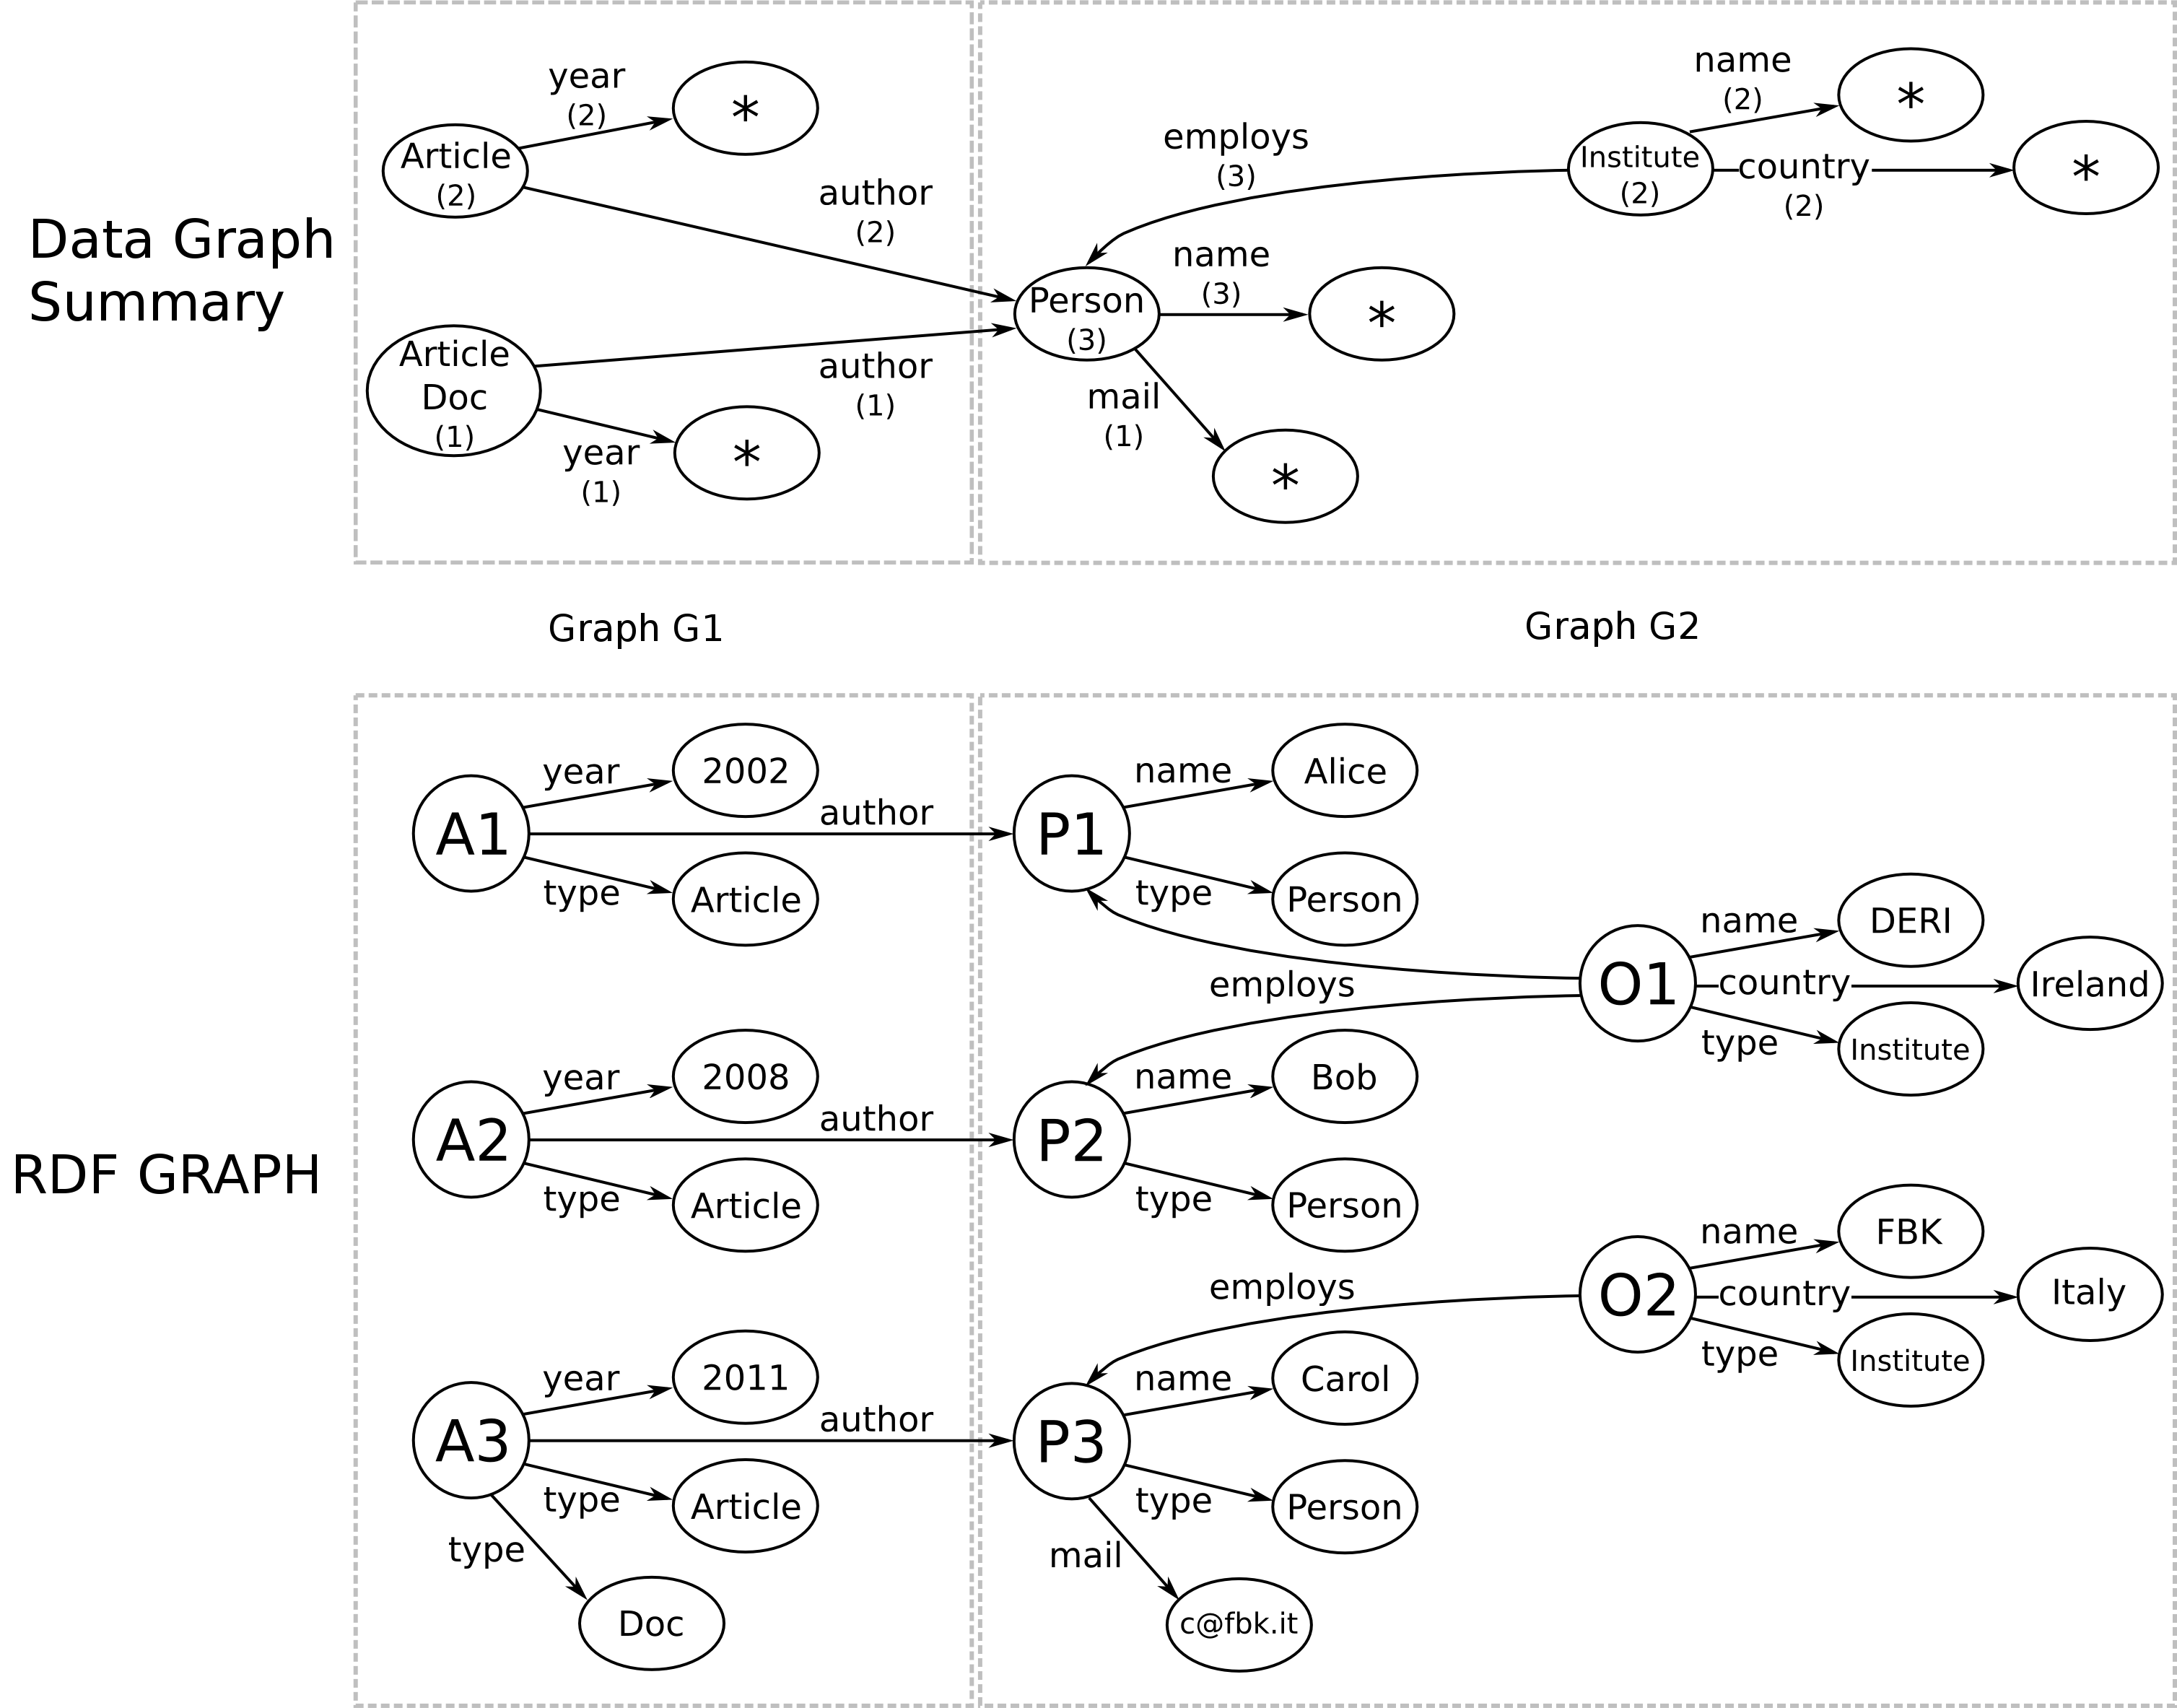
\includegraphics[scale=1]{figures/model.png}}
    \caption{Layers of the Data Graph Summary Model}
    \label{fig:dgs-model}
\end{marginfigure}

The DGS is represented again in RDF using the \emph{Dataset Analytics Vocabulary\footnote{\url{http://vocab.sindice.net/analytics}}} ontology. Usually considerably smaller than the original RDF Graph, it is accessed by the Sparqled via SPARQL. For querying and exploring the DGS outside of SparQLed see the Appendix.

